% !TEX TS-program = xelatex
% !TEX encoding = UTF-8
\documentclass[]{article}
\usepackage{lmodern}
\usepackage{amssymb,amsmath}
\usepackage{ifxetex,ifluatex}
\usepackage{tabularx}
\usepackage{tikz}
\usepackage{fixltx2e} % provides \textsubscript
\ifnum 0\ifxetex 1\fi\ifluatex 1\fi=0 % if pdftex
  \usepackage[T1]{fontenc}
  \usepackage[utf8]{inputenc}
\else % if luatex or xelatex
  \ifxetex
    \usepackage{mathspec}
  \else
    \usepackage{fontspec}
  \fi
  \defaultfontfeatures{Ligatures=TeX,Scale=MatchLowercase}
    \setmainfont[]{AritaM}
\fi
% use upquote if available, for straight quotes in verbatim environments
\IfFileExists{upquote.sty}{\usepackage{upquote}}{}
% use microtype if available
\IfFileExists{microtype.sty}{%
\usepackage{microtype}
\UseMicrotypeSet[protrusion]{basicmath} % disable protrusion for tt fonts
}{}
\usepackage{hyperref}
\hypersetup{unicode=true,
            pdfborder={0 0 0},
            breaklinks=true}
\urlstyle{same}  % don't use monospace font for urls
\usepackage{longtable,booktabs}
\IfFileExists{parskip.sty}{%
\usepackage{parskip}
}{% else
\setlength{\parindent}{0pt}
\setlength{\parskip}{6pt plus 2pt minus 1pt}
}
\setlength{\emergencystretch}{3em}  % prevent overfull lines
\providecommand{\tightlist}{%
  \setlength{\itemsep}{0pt}\setlength{\parskip}{0pt}}
\setcounter{secnumdepth}{0}
% Redefines (sub)paragraphs to behave more like sections
\ifx\paragraph\undefined\else
\let\oldparagraph\paragraph
\renewcommand{\paragraph}[1]{\oldparagraph{#1}\mbox{}}
\fi
\ifx\subparagraph\undefined\else
\let\oldsubparagraph\subparagraph
\renewcommand{\subparagraph}[1]{\oldsubparagraph{#1}\mbox{}}
\fi

\date{}

\begin{document}

\section{이 력 서}

{
\setcounter{tocdepth}{3}
\tableofcontents
}

\clearpage
\subsection{개인정보}

\paragraph{기본정보}

\begin{tabularx}{\textwidth}{@{}XX@{}}
\toprule
Photo & 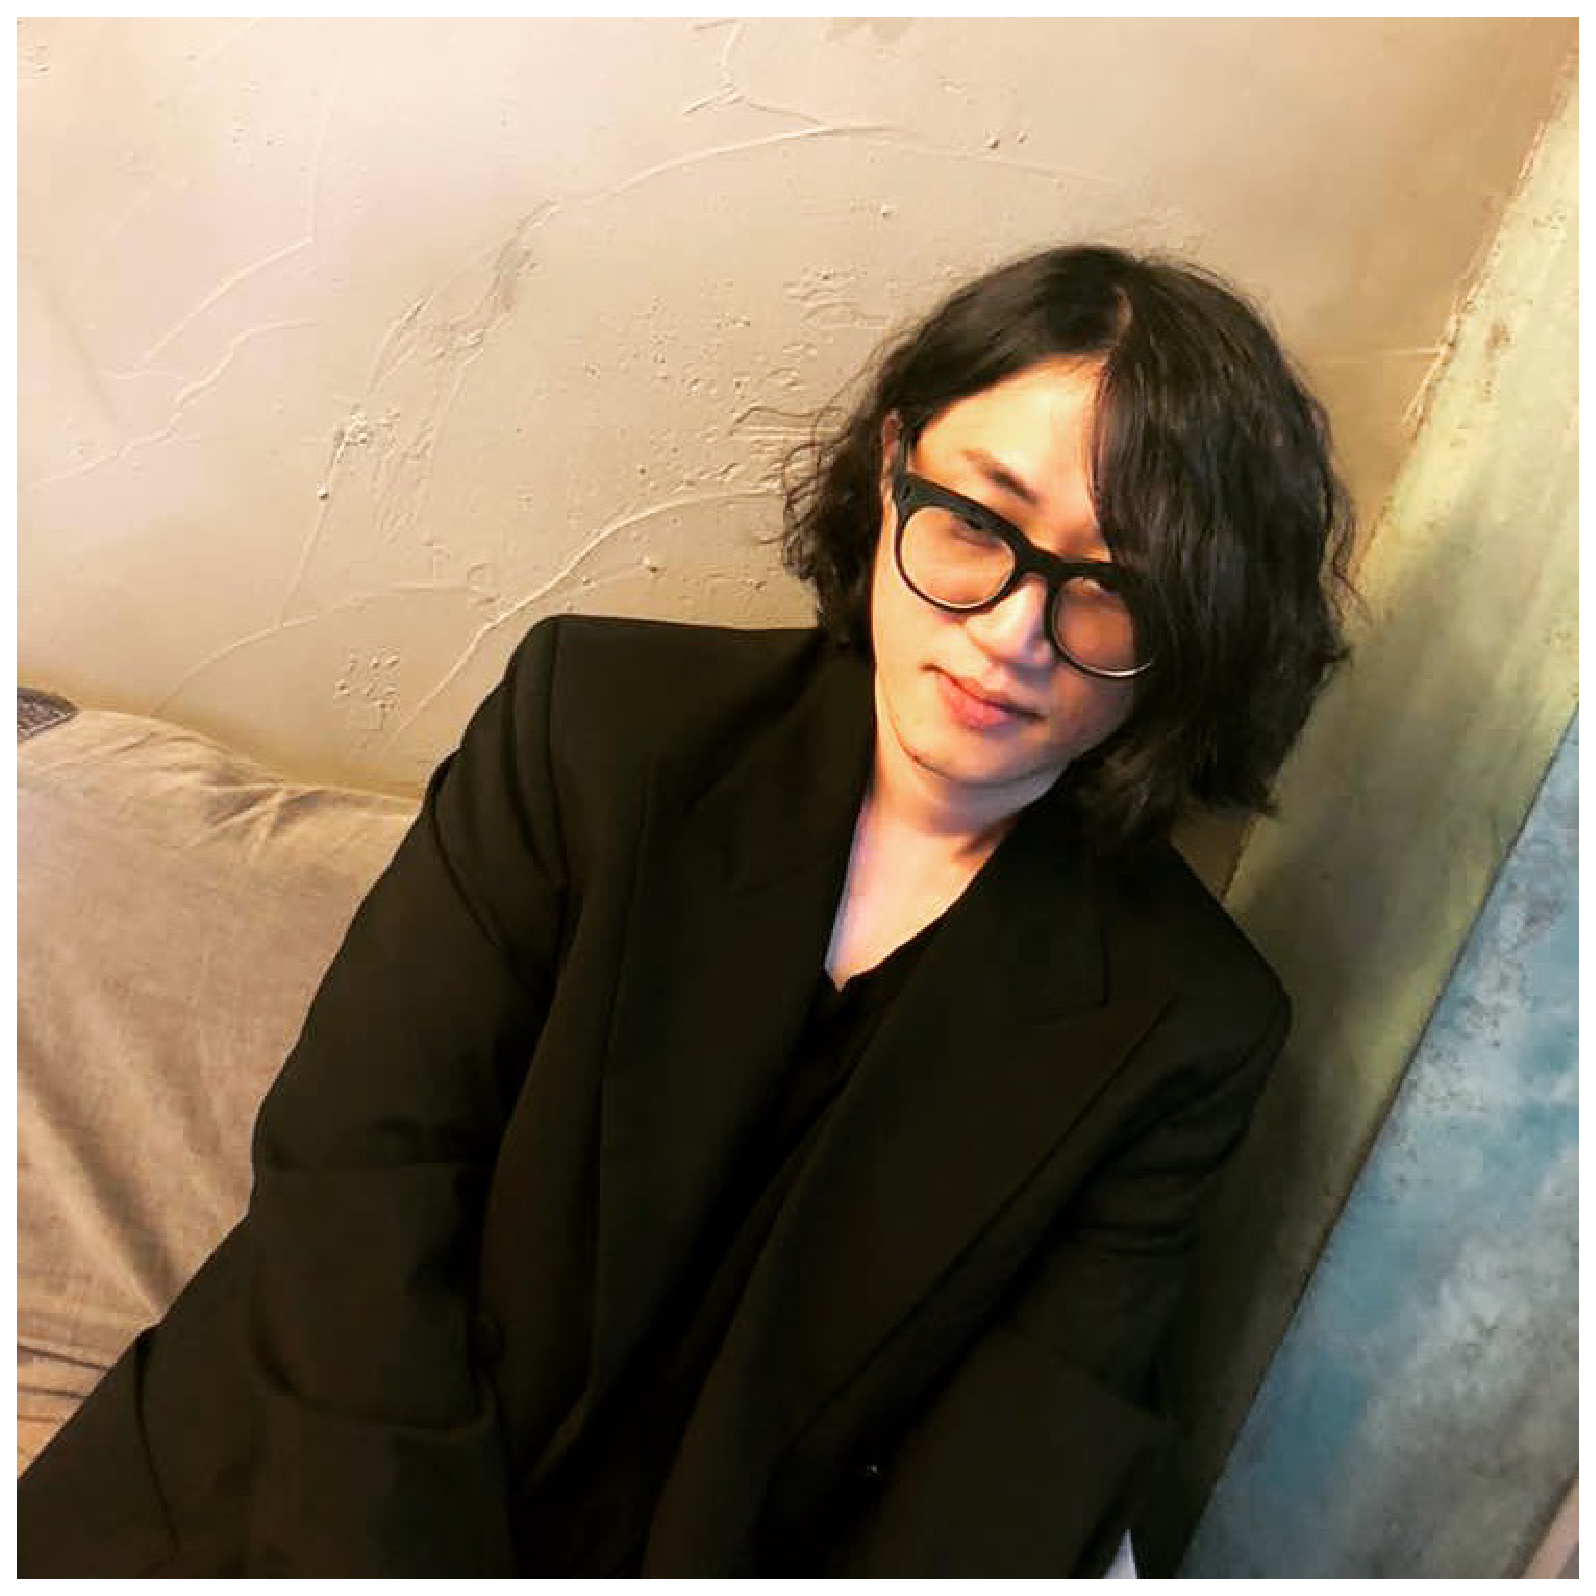
\includegraphics[width=0.30\textwidth]{figure/profile.eps}\\
\midrule
Name & 박은천\\
%- Chinese & 朴恩泉\tabularnewline
- English & Eunchurn Park\\
Age & 36\tabularnewline
Birth Day & 1980.07.05\\
Email & eunchurn.park@gmail.com\\
Mobile & +82-10-4499-6420\\
\bottomrule
\end{tabularx}

%\begin{longtable}[]{@{}ll@{}}
%\toprule
%Photo & {[}{]}(http://eunchurn.com/resume/eunchurn.png ``eunchurn''
%``width:200px'')\tabularnewline
%\midrule
%\endhead
%Name & 박은천\tabularnewline
%%- Chinese & 朴恩泉\tabularnewline
%- English & Eunchurn Park\tabularnewline
%Age & 36\tabularnewline
%Birth Day & 1980.07.05\tabularnewline
%Email & eunchurn.park@gmail.com\tabularnewline
%Mobile & +82-10-4499-6420\tabularnewline
%\bottomrule
%\end{longtable}

\paragraph{신상정보}

\begin{tabularx}{\textwidth}{@{}XX@{}}
\toprule
Profile & Content\\
\midrule
Address & 서울시 구로구 경인로 619-3 신도림3차푸르지오 아파트
1103호\\
Mobile & 010-4499-6420\\
Married & 기혼\\
%Family & 부모형\tabularnewline
%Blood type & RH+ B\tabularnewline
%Religion & 기독교\tabularnewline
\bottomrule
\end{tabularx}


%\begin{longtable}[]{@{}ll@{}}
%\toprule
%Profile & Content\tabularnewline
%\midrule
%\endhead
%Address & 서울시 구로구 경인로 619-3 신도림3차푸르지오 아파트
%1103호\tabularnewline
%Mobile & 010-4499-6420\tabularnewline
%Married & 기혼\tabularnewline
%%Family & 부모형\tabularnewline
%%Blood type & RH+ B\tabularnewline
%%Religion & 기독교\tabularnewline
%\bottomrule
%\end{longtable}

\paragraph{학력정보}

\begin{tabularx}{\textwidth}{@{}XXXXXX@{}}
\toprule
Level & School Name & Major & Start & End & Status\\
\midrule
Ph.D. & 단국대학교 대학원& 건축공학과 건축구조 &
2007.03.01 & 2017.08.23 & graduated \\
M.S. & 단국대학교 대학원& 건축공학과 건축구조 &
2005.03.01 & 2007.02.14 & graduated \\
B.S. & 단국대학교& 건축공학과 & 1999.03.02 &
2005.02.18 & graduated \\
\bottomrule
\end{tabularx}

%\begin{longtable}[]{lllllll}
%\toprule
%Level & School Name & Major & Start & End & Status\tabularnewline
%\midrule
%\endhead
%Ph.D Candidate & 단국대학교 대학원& 건축공학과 건축구조 &
%2007.03.01 & 2013.02.14 & completion \tabularnewline
%M.S. & 단국대학교 대학원& 건축공학과 건축구조 &
%2005.03.01 & 2007.02.14 & graduated \tabularnewline
%B.S. & 단국대학교& 건축공학과 & 1999.03.02 &
%2005.02.18 & graduated \tabularnewline
%\bottomrule
%\end{longtable}

\subsection{직장이력}

\begin{tabularx}{\textwidth}{@{}XXX@{}}
\toprule
Period & Company & Part \textgreater{} Team\\
\midrule
2004.10 - 2009.4 & \href{http://www.srrc.re.kr/}{단국대학교 부설
리모델링연구소} & R\&D \textgreater{} 구조해석 및 동역학\\
2009.04 - 2015.5 & \href{http://www.kmbest.co.kr/}{한국유지관리(주)} &
부설기업연구소 R\&D \textgreater{} U사업팀 토목/건축
계측/해석\\
2015.08 - 현재 & \href{http://www.shtpi.co.kr/}{승화기술정책연구소(주)}
& 기업연구소 R\&D \textgreater{} 영상처리/M2M/철도과제\\
\bottomrule
\end{tabularx}


%\begin{longtable}[]{@{}lll@{}}
%\toprule
%Period & Company & Part \textgreater{} Team\tabularnewline
%\midrule
%\endhead
%2004.10 - 2009.4 & \href{http://www.srrc.re.kr/}{단국대학교 부설
%리모델링연구소} & R\&D \textgreater{} 구조해석 및 동역학\tabularnewline
%2009.04 - 2015.5 & \href{http://www.kmbest.co.kr/}{한국유지관리(주)} &
%부설기업연구소 R\&D \textgreater{} U사업팀 토목/건축
%계측/해석\tabularnewline
%2015.08 - 현재 & \href{http://www.shtpi.co.kr/}{승화기술정책연구소(주)}
%& 기업연구소 R\&D \textgreater{} M2M/자산관리\tabularnewline
%\bottomrule
%\end{longtable}

\subsection{프로그램 스킬}
\begin{tabularx}{\textwidth}{@{}XX@{}}
\begin{tikzpicture}
\node [anchor=west] at (0,1) {Analysis : Mathworks MATLAB};
\draw [fill=gray!50] (0,0) rectangle (5,.5);
\draw [fill={rgb:red,1;green,2;blue,3}] (0,0) rectangle (4.5,.5);
\end{tikzpicture}
&
\begin{tikzpicture}
\node [anchor=west] at (0,1) {Analysis \& Control : Mathworks Simulink};
\draw [fill=gray!50] (0,0) rectangle (5,.5);
\draw [fill={rgb:red,1;green,2;blue,3}] (0,0) rectangle (4.5,.5);
\end{tikzpicture}
\\
\begin{tikzpicture}
\node [anchor=west] at (0,1) {Control : National Instruments LabVIEW};
\draw [fill=gray!50] (0,0) rectangle (5,.5);
\draw [fill={rgb:red,1;green,2;blue,3}] (0,0) rectangle (4.0,.5);
\end{tikzpicture}
&
\begin{tikzpicture}
\node [anchor=west] at (0,1) {Documentation : LaTeX, XeLaTex, Beamer};
\draw [fill=gray!50] (0,0) rectangle (5,.5);
\draw [fill={rgb:red,1;green,2;blue,3}] (0,0) rectangle (4.0,.5);
\end{tikzpicture}
\\
\begin{tikzpicture}
\node [anchor=west] at (0,1) {\begin{tabular}{l}Front-end development : \\Javascript/HTML5/Angularjs/Bootstrap\end{tabular}};
\draw [fill=gray!50] (0,0) rectangle (5,.5);
\draw [fill={rgb:red,3;green,1;blue,2}] (0,0) rectangle (3.0,.5);
\end{tikzpicture}
&
\begin{tikzpicture}
\node [anchor=west] at (0,1) {\begin{tabular}{l}Back-end development : \\Nodejs/Python\end{tabular}};
\draw [fill=gray!50] (0,0) rectangle (5,.5);
\draw [fill={rgb:red,1;green,0;blue,0}] (0,0) rectangle (4.0,.5);
\end{tikzpicture}
\\
\begin{tikzpicture}
\node [anchor=west] at (0,1) {\begin{tabular}{l}Communication development : \\WebSocket,RS-232\end{tabular}};
\draw [fill=gray!50] (0,0) rectangle (5,.5);
\draw [fill={rgb:red,1;green,0;blue,0}] (0,0) rectangle (4.0,.5);
\end{tikzpicture}
&
\begin{tikzpicture}
\node [anchor=west] at (0,1) {\begin{tabular}{l}DB build : \\ NoSQL (mongoDB, Redis,...), MySQL, Oracle\end{tabular}};
\draw [fill=gray!50] (0,0) rectangle (5,.5);
\draw [fill={rgb:red,1;green,0;blue,0}] (0,0) rectangle (3.0,.5);
\end{tikzpicture}
\\
\begin{tikzpicture}
\node [anchor=west] at (0,1) {\begin{tabular}{l}Server Build : AWS (EC2, Route53, \\Cloudfront, ELB,...), Raspberry Pi, Ubuntu 16.04\end{tabular}};
\draw [fill=gray!50] (0,0) rectangle (5,.5);
\draw [fill={rgb:red,1;green,0;blue,0}] (0,0) rectangle (3,.5);
\end{tikzpicture}
&
\begin{tikzpicture}
\node [anchor=west] at (0,1) {Shell script : Bash (Debian based Linux)};
\draw [fill=gray!50] (0,0) rectangle (5,.5);
\draw [fill={rgb:red,1;green,0;blue,0}] (0,0) rectangle (3,.5);
\end{tikzpicture}
\\
\begin{tikzpicture}
\node [anchor=west] at (0,1) {Tools \& VM : Git/Slack/Docker};
\draw [fill=gray!50] (0,0) rectangle (5,.5);
\draw [fill={rgb:red,1;green,0;blue,0}] (0,0) rectangle (3,.5);
\end{tikzpicture}
&
\begin{tikzpicture}
\node [anchor=west] at (0,1) {ETC : Adobe Photoshop/Illustrator/After Effect/...};
\draw [fill=gray!50] (0,0) rectangle (5,.5);
\draw [fill={rgb:red,0;green,1;blue,0}] (0,0) rectangle (3.0,.5);
\end{tikzpicture}
\\
\end{tabularx}
%\begin{tikzpicture}
%\node [anchor=west] at (.1,.8) {Ableton Live};
%\draw [fill=gray!50] (0,0) rectangle (5,.5);
%\draw [fill={rgb:red,0;green,1;blue,0}] (0,0) rectangle (5.0,.5);
%\end{tikzpicture}



\subsection{프로젝트 수행이력(석박사과정 제외)}

\subsubsection{초고층 건물의 \href{http://gnss.ngii.go.kr/info/summary}{GNSS} 망조정기법과 외란보정 기법을 이용한 거푸집 연직도 관리}

\begin{itemize}
\item
  소개 \textgreater{} 초고층건물 시공에서
  \href{http://gnss.ngii.go.kr/info/summary}{GNSS}를 이용하여 연직도를
  관리하고자 하는 신기술 인증 프로젝트, 거푸집 연직도 시공 누적오차
  10mm이내 / 시공 층별오차 4mm 이내의 관리기준을 만족해야 함.
\item
  실제 수행한 주요 이력 \textgreater{} *
  \href{https://en.wikipedia.org/wiki/Real_Time_Kinematic}{RTK}-\href{https://en.wikipedia.org/wiki/Virtual_Reference_Station}{VRS}\footnote{Virtual
    Reference Station (VRS) networks use real-time kinematic (RTK)
    solutions to provide high-accuracy, RTK Global Navigation Satellite
    Systems.} 시공 \textgreater{} * 기준점 네트워크 망조정 : 기준국을
  타설하여 3점, 4점
  \href{https://en.wikipedia.org/wiki/Procrustes_analysis}{Procrustes}기법을
  사용하여 망조정 : OPA\footnote{\href{https://en.wikipedia.org/wiki/Procrustes_analysis}{Ordinary
    Procrustes Analysis (OPA)}} 방식으로 1초단위의 scale, rotation값을
  생성하여 값보정 \textgreater{} * 센서퓨전(Sensor fusion) : 가속도계를
  설치하여
  \href{http://scholar.lib.vt.edu/theses/available/etd-062899-064821/unrestricted/etd.PDF}{Multirate-Kalman
  Filter (MR-KF)}\footnote{\href{http://scholar.lib.vt.edu/theses/available/etd-062899-064821/unrestricted/etd.PDF}{Multirate-Kalman
    Filter (MR-KF)}} 사용으로 거푸집의 고속변위예측 \textgreater{} *
  네트워크 망조정 필터 : 망조정기법에서 scale값과 roation값을 Kalman
  Filter\footnote{\href{https://ko.wikipedia.org/wiki/\%EC\%B9\%BC\%EB\%A7\%8C_\%ED\%95\%84\%ED\%84\%B0}{칼만
    필터(Kalman filter)}는 잡음이 포함되어 있는 선형 역학계의 상태를
    추적하는 재귀 필터로, 루돌프 칼만이 개발하였다. 칼만 필터는 컴퓨터
    비전, 로봇 공학, 레이더 등의 여러 분야에 사용되며, 많은 경우에 매우
    효율적인 성능을 보여준다.}로 수정 \textgreater{} * 초기
  개발단계에서의 개발내용을 전면수정하여 상위의 모든 기술을 적용함
\item
  적용된 기술 \textgreater{} *
  \href{http://gnss.ngii.go.kr/info/summary}{GNSS}\footnote{\href{http://gnss.ngii.go.kr/info/summary}{GNSS(Global
    Navigation Satellite System)}는 위성을 이용한 전파항법 시스템으로,
    수십 개의 위성을 이용하여 전 세계의 모든 지역에서 언제든지 위치와
    시각 서비스 제공이 가능할 뿐만 아니라 수신기 가격이 저렴하며 오차가
    작기 때문에 응용범위가 매우 다양하다.} (GPS, Glonass) System :
  \href{http://www.septentrio.com/}{Septentrio} GNSS 적용 \textgreater{}
  * RF 통신 : 각 기준점의 GNSS와 통신 \textgreater{} *
  \href{https://en.wikipedia.org/wiki/Differential_GPS}{Real-time
  Kinematic Method (DGPS)} \textgreater{} *
  \href{https://en.wikipedia.org/wiki/Procrustes_analysis}{Ordinary
  Procrustes Analysis (OPA)} \textgreater{} *
  \href{http://scholar.lib.vt.edu/theses/available/etd-062899-064821/unrestricted/etd.PDF}{Multirate-Kalman
  Filter (MR-KF)} \textgreater{} *
  \href{http://ieeexplore.ieee.org/xpl/login.jsp?tp=\&arnumber=258116\&url=http\%3A\%2F\%2Fieeexplore.ieee.org\%2Fxpls\%2Fabs_all.jsp\%3Farnumber\%3D258116}{Fourier
  Linear Combiner (FLC)}\footnote{\href{http://ieeexplore.ieee.org/xpl/login.jsp?tp=\&arnumber=258116\&url=http\%3A\%2F\%2Fieeexplore.ieee.org\%2Fxpls\%2Fabs_all.jsp\%3Farnumber\%3D258116}{Fourier
    Linear Combiner, FLC} : A tuning of the algorithm parameters and a
    sensitivity analysis to its initial conditions was performed using
    treadmill walking data from 3 healthy subjects. The accuracy of the
    method was then assessed using data collected from 15 young healthy
    subjects during treadmill walking at variable speeds and comparing
    the pitch, roll, and yaw angles estimated from the gyroscopes data
    to those obtained with a stereophotogrammetric system. Root mean
    square (RMS) difference and correlation coefficients (r) were used
    for this purpose.}
\item
  개발 S/W 플랫폼 \textgreater{} *
  \href{https://en.wikipedia.org/wiki/National_Instruments}{National
  Instruments} \href{https://en.wikipedia.org/wiki/LabVIEW}{LabVIEW}
  \textgreater{} *
  \href{https://en.wikipedia.org/wiki/MathWorks}{Mathworks}
  \href{https://en.wikipedia.org/wiki/MATLAB}{MATLAB}
\item
  참여한 현장 \textgreater{} * 마포 주상복합 : 후처리
  \href{https://en.wikipedia.org/wiki/Differential_GPS}{DGPS} 시스템
  적용 \textgreater{} * 롯데슈퍼타워 브레이스 위치 측정 : GNSS-RTK만
  적용 \textgreater{} * 현대제철 당진 코크스 연돌
  \href{https://en.wikipedia.org/wiki/Climbing_formwork}{ACS거푸집}\footnote{The
    Automatic Climbing System (ACS) is a hydraulically operated
    self-climbing formwork system used for the construction of tall
    concrete structures such as building core walls and bridge pylons.
    Tall concrete structures have historically been formed with crane
    lifted formwork often referred to as ``jump'' forms. These systems
    require a worker to ride the formwork as it is raised to its next
    position in order to insert reties through the previously cast lift
    to secure the form. This procedure requires extensive crane time and
    is too slow, unsafe and unproductive for tall structures where the
    concrete walls are typically on the critical path.} 계측 : 3점망조정
  RTK적용 \textgreater{} * 부산 연산구 거제동 롯데캐슬피렌체 주상복합
  건물 거푸집계측 : 3점망조정, 4점망조정 데이터 (실제 거푸집 시공에
  반영) \textgreater{} * 인천 청라지구 롯데케슬 주상복합 건물 거푸집
  계측 : 4점망조정 데이터 (신기술 현장실사) \textgreater{} * 인천
  청라지구 롯데케슬 주상복합 건물 거푸집 계측 :
  \href{http://scholar.lib.vt.edu/theses/available/etd-062899-064821/unrestricted/etd.PDF}{MR-KF}
  시범적용
\item
  개발결과 : 건설신기술인증
  \href{http://www.kaia.re.kr/portal/newtec/view.do?searchCnd=1\&searchWrd=\&menuNo=200075\&frApntYear=\&toApntYear=\&pageUnit=10\&frApntNo=\&toApntNo=\&cate1=\&cate2=\&cate3=\&tecCat1=\&tecCat2=\&tecCat3=\&newtecCat1=\&newtecCat2=\&newtecCat3=\&dvlprNm=\%ED\%95\%9C\%EA\%B5\%AD\%EC\%9C\%A0\%EC\%A7\%80\%EA\%B4\%80\%EB\%A6\%AC\&ordDvs=\&pageIndex=1\&apntNo=625\&frMenu=list}{국토해양부고시
  제2011 -313호}
\end{itemize}

\subsubsection{코레일 공항철도 및 KTX 진동가속도 분석 시스템}

\begin{itemize}
\item
  소개 \textgreater{} 차축-대차-차체의 좌우 2방향 가속도계 설치, 차축의
  타코미터 설치, 계측시스템을 구성하여 공항철도의 궤도이상개소검출,
  열차의 주행안정성평가,
  \href{http://ieeexplore.ieee.org/xpl/login.jsp?tp=\&arnumber=264942\&url=http\%3A\%2F\%2Fieeexplore.ieee.org\%2Fxpls\%2Fabs_all.jsp\%3Farnumber\%3D264942}{slip/slide}
  및 승차감평가 시스템 개발 및 준공
\item
  실제 수행한 주요 이력 \textgreater{} * 공항철도 이상개소 분석시스템 :
  10m KP간격 CWA-FRF\footnote{Coherence Weighted Averaged Frequency
    Response Function (CWA-FRF) refer to
    ``\href{http://institute.lanl.gov/ei/shm/pubs/modal_stat_jvc_jul00.pdf}{Estimation
    Of Statistical Distributions For Modal Parameters Identified From
    Averaged Frequency Response Function Data}'', Journal of Vibration
    and Control, July 2000} 함수로 전달함수 예측, 측정된
  차축-대차-차체의
  \href{https://en.wikipedia.org/wiki/Frequency_response}{주파수응답함수(Frequency
  response function, FRF)}를 통해 중심주파수-대역폭-가중치함수를 규정,
  \href{http://www.scholarpedia.org/article/Boundary_value_problem}{경계비선형}
  최적화 알고리즘 적용으로 이상개소 분석시스템 구축 \textgreater{} *
  공항철도 차량 주행 안정성 분석 시스템 : 병진, 롤링진동 분석 후
  속도/도상 별 기준값 적용하여 이상진동의 위치 검출 \textgreater{} *
  공항철도/도시철도 승차감 분석 시스템 :
  \href{http://www.iso.org/iso/catalogue_detail.htm?csnumber=7612}{ISO
  2631-1:1997}과
  \href{http://www.uic.org/etf/codex/codex-detail.php?codeFiche=513\&langue_fiche=E}{UIC513}에서
  제시한 방법으로 각각 필터제작 4채널 DAQ보드와 3축 가속도계 센서 적용
  \textgreater{} * 공항철도 slip/slide : 타코미터의 펄스의 계측노이즈
  정규화 제거하고 속도 수치미분으로 임계값으로 정성적으로 판단. 실제
  주행거리와 slip/slide 개소와 그 거리는 대부분 일치함으로 확인.
  \textgreater{} * KTX 주행거동평가 알고리즘 : 국내에서 개발한 KTX산천,
  각 분기기등 분석,
  \href{http://www.uic.org/etf/codex/codex-detail.php?langue_fiche=E\&codeFiche=518}{UIC-518OR}
  기준에 따라 주행거동평가, 누적분포 활용해서 99.85\% 0.15\%의 피크 검출
\item
  적용된 기술 \textgreater{} * Coherence-weighted Averaging Frequency
  Response Function Estimation \textgreater{} * Fast Algorithm for
  Nonlinearly Constrained Optimization Calculations \textgreater{} *
  \href{https://en.wikipedia.org/wiki/Finite_impulse_response}{FIR
  Filter} design
\item
  개발 S/W 플랫폼 \textgreater{} * Mathworks MATLAB / GUI
\item
  참여한 현장 \textgreater{} * 코레일 공항철도 (인천-김포)
  \textgreater{} * 도시철도공사 5호선 (승차감분석, Comfort analysis)
  \textgreater{} * 코레일 KTX (서울-부산구간)
\end{itemize}

\subsubsection{LCD Display 글래스 이송로봇진동 사전감지시스템 (\href{https://en.wikipedia.org/wiki/Early_warning_system}{Early Warning System})}

\begin{itemize}
\item
  소개 \textgreater{} Glass를 옮기는 이송로봇에 3축가속도계 1기 설치하여
  로봇관절운동의 패턴을 분류하고 초기치에 비해 변화량을 모니터링 해서 각
  파트의 이상을 미리 감지. 제조사측은
  사전진단(\href{https://en.wikipedia.org/wiki/Early_warning_system}{Eearly
  Warning System, EWS})과 부품별
  파트진단(\href{https://en.wikipedia.org/wiki/Predictive_maintenance}{Prediction
  Management Program, PMP})을 수행하기 원함.
\item
  실제 수행한 주요 이력 \textgreater{} * 신호분리기법 적용 :
  \href{https://en.wikipedia.org/wiki/Hankel_matrix}{Hankel Matrix}와
  \href{https://en.wikipedia.org/wiki/Singular_value_decomposition}{Singular
  value decomposition, SVD}기법을 활용해서 signal decomposition 적용
  그리고 \href{https://en.wikipedia.org/wiki/Wavelet}{wavelet} 기법을
  적용해서 신호분리도 적용 \textgreater{} * 패턴분류 :
  rms-triggering기법으로 구간을 나눈후
  \href{https://en.wikipedia.org/wiki/Independent_component_analysis}{ICA(independent
  component analysis)}적용 \textgreater{} * Spectrogram과 Cepstrum
  분석으로 사전진단 가능성 판단 \textgreater{} * 각관절의 기어박스,
  rotor의 엔코더 데이터를 받아서 order-analysis 를 수행하여야 정확한
  파트이상진단까지 할 수 있었으나 비용등의 문제로 더이상 진행하지 못함.
  \textgreater{} * 중소기업 과제로 변경 수행완료
\item
  적용된 기술 \textgreater{} * Hankel matrix based signal
  decomposition\footnote{The linear sum of a series of component signals
    by Hankel matrix-based SVD, and essentially what the component
    signals reflect are projections of original signal on the
    orthonormal bases of m-dimensional and n-dimensional vector spaces.
    Refer to Xuezhi Zhao, , Bangyan Ye(2009),
    ``\href{http://www.sciencedirect.com/science/article/pii/S0888327008002604}{Similarity
    of signal processing effect between Hankel matrix-based SVD and
    wavelet transform and its mechanism analysis}'', \emph{Mechanical
    Systems and Signal Processing} Volume 23, Issue 4, May 2009, Pages
    1062--1075} \textgreater{} * Wavelet analysis \textgreater{} *
  \href{https://en.wikipedia.org/wiki/Independent_component_analysis}{Independent
  component analysis} \textgreater{} *
  \href{https://en.wikipedia.org/wiki/Cepstrum}{Cepstrum
  analysis}\footnote{A cepstrum is the result of taking the Inverse
    Fourier transform (IFT) of the logarithm of the estimated spectrum
    of a signal.} \textgreater{} *
  \href{https://en.wikipedia.org/wiki/Spectrogram}{Spectrogram}\footnote{A
    spectrogram is a visual representation of the spectrum of
    frequencies in a sound or other signal as they vary with time or
    some other variable.} / Order-analysis\footnote{\href{http://zone.ni.com/reference/en-XX/help/372416A-01/svtconcepts/intro_ord_ana/}{Order
    analysis} is a technique for analyzing sound and vibration signals
    from rotating or reciprocating machinery, such as engines,
    compressors, turbines, and pumps. These machines have a variety of
    parts, and each part contributes unique sound and vibration patterns
    to the sound and vibration pattern of the whole machine. With order
    analysis, you can identify and isolate these sound and vibration
    patterns to analyze the performance and quality of each machine part
    individually.}
\item
  개발 S/W 플랫폼 \textgreater{} * Mathworks MATLAB / GUI
\item
  참여한 현장 \textgreater{} * LG Display 파주공장
\end{itemize}

\subsubsection{초고층건물 구조건전도 모니터링}\href{https://en.wikipedia.org/wiki/Structural_health_monitoring}{Structural Health Monitoring}\footnote{The process of implementing a damage detection and characterization strategy for engineering structures is referred to as \href{https://en.wikipedia.org/wiki/Structural_health_monitoring}{Structural Health Monitoring (SHM)}}
\begin{itemize}
\item
  소개 \textgreater{} 초고층건물의 시공중/사용중 계측 모니터링 : 주로
  FBG, 지진가속도계, 가속도계, GPS, 풍향풍속계 사용.
\item
  실제 수행한 주요 이력 \textgreater{} *
  \href{https://en.wikipedia.org/wiki/Signal-to-noise_ratio}{SNR}
  125dB\textasciitilde{}130dB 이상의 센서에 적합한
  \href{https://en.wikipedia.org/wiki/Data_acquisition}{DAQ} 보드 개발 :
  저주파와 신호대잡음비 성능이 우수한 가속도계 센서에 적합한
  \href{https://en.wikipedia.org/wiki/Data_acquisition}{DAQ}는 사실상
  고가임. 따라서 설치가 용이한 유선 네트워크방식의
  \href{https://en.wikipedia.org/wiki/Data_acquisition}{DAQ}보드 개발이
  필요하여 개발참여.
  \href{http://kr.mathworks.com/help/daq/examples/getting-started-with-session-based-interface-using-ni-devices.html}{Session-based
  interface} 프로그래밍으로 데이터수집을 다른 thread로 작동시킴과 동시에
  분석과 해석이 동시에 이루어짐 (실시간 모드벡터 추출/FFT또는
  파워스펙트럼 그래프도시) \textgreater{} * 시각동기화 프로토콜 적용
  \href{https://ko.wikipedia.org/wiki/IEEE_1588}{IEEE-1588 Precision
  Time Protocol}\footnote{Precision Time Protocol(PTP)은 네트워크 간
    정확한 동기화를 가능케하는
    \href{https://ko.wikipedia.org/wiki/IEEE_1588}{IEEE 1588} 표준 시간
    전송 프로토콜이다.하드웨어에서 생성하는 타임스탬프를 사용할 때
    나노초 단위의 정확도까지 보장해 준다.} : GPS 클럭을 모든 장비에
  연결하려면 많은 인력과 비용이 소모됨. 따라서 유선네트워크 방식에서의
  동기화 프로토콜을 적용 (펌웨어단계에서 클럭동기화에 성공)
  \textgreater{} * 지진경보 시스템 : 여러동의 건물의 경우 각동 지하에
  지진가속도계를 설치하여 지진경보를 발령. 이때 각동의 EPGA\footnote{In
    seismic engineering, the effective peak acceleration (EPA, the
    maximum ground acceleration to which a building responds) is often
    used, which tends to be ⅔ -- ¾ the PGA, The term
    `\href{http://www.teachmefinance.com/Scientific_Terms/Effective\%20peak\%20ground\%20acceleration.html\#ixzz3iNuQcQLs}{Effective
    peak ground acceleration}' as it applies to the area of reclamation
    can be defined as `That acceleration which is most closely related
    to structural response and to damage potential of an earthquake'.}값으로
  rms-triggering 적용 각 3개의 동에서 동시에 임계값 이상이 발생하였을 때
  지진으로 판정. \textgreater{} * 모드정보 추출 : SSI(Stochastic
  subspace identification)\footnote{The data driven
    \href{http://www.svibs.com/solutions/literature/2006_2.pdf}{\textbf{Stochastic
    Subspace Identification}} techniques is considered to be the most
    powerful class of the known identification techniques for natural
    input modal analysis in the time domain. Refer to B. Peeters and G.
    D. Rodeck (1999),
    ``\href{ftp://193.136.28.78/pub/Personal/Dec/filipema/public/FCT_WindOMA/ref_8.pdf}{Reference-based
    Stochastic Subspace Identification for Output-only Modal
    Analysis}'', \emph{Mechanical Systems and Signal Processing} (1999)
    13(6), 855\}878} 기법과
  \href{https://en.wikipedia.org/wiki/Frequency_domain_decomposition}{FDD(Frequency
  domain decomposition)}\footnote{The
    \href{https://en.wikipedia.org/wiki/Frequency_domain_decomposition}{frequency
    domain decomposition (FDD)} is an output-only system identification
    technique popular in civil engineering, in particular in structural
    health monitoring. As an output-only algorithm, it is useful when
    the input data is unknown. FDD is a modal analysis technique which
    generates a system realization using the frequency response given
    (multi-)output data} 기법을 적용
\item
  적용된 기술 \textgreater{} *
  \href{http://kr.mathworks.com/products/daq/}{Data acquisition toolbox
  (MATLAB)} \textgreater{} *
  \href{https://ko.wikipedia.org/wiki/IEEE_1588}{IEEE-1588 Precision
  Time Protocol} \textgreater{} * High-Resolution Analog-To-Digital
  Conversion \textgreater{} * Stochastic subspace identification
  \textgreater{} * Frequency domain decomposition \textgreater{} *
  \href{https://en.wikipedia.org/wiki/Eigensystem_realization_algorithm}{Eigensystem
  Realization Algorithm} \textgreater{} *
  \href{https://en.wikipedia.org/wiki/Finite_element_updating}{FE Model
  update}\footnote{\href{https://en.wikipedia.org/wiki/Finite_element_updating}{Finite
    element model updating} is the process of ensuring that finite
    element analysis results in models that better reflect the measured
    data than the initial models. It is part of verification and
    validation of numerical models.} /
  \href{https://en.wikipedia.org/wiki/System_identification}{System
  Identification}\footnote{The field of
    \href{https://en.wikipedia.org/wiki/System_identification}{system
    identification} uses statistical methods to build mathematical
    models of dynamical systems from measured data. System
    identification also includes the optimal design of experiments for
    efficiently generating informative data for fitting such models as
    well as model reduction.}
\item
  개발 S/W 플랫폼 \textgreater{} * Mathworks MATLAB / GUI
\item
  참여한 현장 \textgreater{} * 부산 해운대 두산위브더제니스 (사용중계측
  SHM) \textgreater{} * 인천 송도 NEATT 동북아무역센터 (시공중계측)
  \textgreater{} * 롯데 잠실 슈퍼타워 (RFP지원\&자문) \textgreater{} * 송도 M1
  주상복합 (자문)
\end{itemize}

%\subsubsection{능동형 제진장치 (\href{http://www.sciencedirect.com/science/article/pii/S0141029697000722}{Active \& Hybrid Mass Damper, A-HMD}) 프로젝트}
%%(\href{http://www.sciencedirect.com/science/article/pii/S0141029697000722}{Active \& Hybrid Mass Damper, A-HMD}
%\begin{itemize}
%\item
%  소개 \textgreater{} 건물의 사용중 진동 저감을 위한 능동형 제진장치
%  설치 프로젝트
%\item
%  실제 수행한 주요 이력 \textgreater{} *
%  \href{http://www.quanser.com/products/active_mass_damper}{Quansar 소형
%  AMD 제어},
%  \href{https://en.wikipedia.org/wiki/Linear-quadratic_regulator}{LQR}\footnote{The
%    theory of optimal control is concerned with operating a dynamic
%    system at minimum cost. The case where the system dynamics are
%    described by a set of linear differential equations and the cost is
%    described by a quadratic function is called the LQ problem. One of
%    the main results in the theory is that the solution is provided by
%    the
%    \href{https://en.wikipedia.org/wiki/Linear-quadratic_regulator}{linear-quadratic
%    regulator (LQR)}, a feedback controller whose equations are given
%    below. The
%    \href{https://en.wikipedia.org/wiki/Linear-quadratic_regulator}{LQR}
%    is an important part of the solution to the
%    \href{https://en.wikipedia.org/wiki/Linear-quadratic-Gaussian_control}{LQG
%    (Linear-Quadratic-Gaussian)} problem. Like the
%    \href{https://en.wikipedia.org/wiki/Linear-quadratic_regulator}{LQR}
%    problem itself, the
%    \href{https://en.wikipedia.org/wiki/Linear-quadratic-Gaussian_control}{LQG}
%    problem is one of the most fundamental problems in control theory.}/\href{https://en.wikipedia.org/wiki/Linear-quadratic-Gaussian_control}{LQG}\footnote{In
%    control theory, the
%    \href{https://en.wikipedia.org/wiki/Linear-quadratic-Gaussian_control}{linear-quadratic-Gaussian
%    (LQG)} control problem is one of the most fundamental optimal
%    control problems. It concerns uncertain linear systems disturbed by
%    additive white Gaussian noise, having incomplete state information
%    (i.e.~not all the state variables are measured and available for
%    feedback) and undergoing control subject to quadratic costs.
%    Moreover the solution is unique and constitutes a linear dynamic
%    feedback control law that is easily computed and implemented.
%    Finally the
%    \href{https://en.wikipedia.org/wiki/Linear-quadratic-Gaussian_control}{LQG}
%    controller is also fundamental to the optimal control of perturbed
%    non-linear systems.} 알고리즘 탑재. \textgreater{} * 실제 현장에서
%  계측데이터 품질 확보를 위한 signal conditioning \textgreater{} *
%  High-resolution DAQ 적용
%\item
%  적용된 기술 \textgreater{} *
%  \href{https://en.wikipedia.org/wiki/Linear-quadratic_regulator}{LQR}/\href{https://en.wikipedia.org/wiki/Linear-quadratic-Gaussian_control}{LQG}
%  control algorithm \textgreater{} *
%  \href{https://en.wikipedia.org/wiki/Sliding_mode_control}{sliding mode
%  control}\footnote{In control system,
%    \href{https://en.wikipedia.org/wiki/Sliding_mode_control}{sliding
%    mode control, or SMC}, is a nonlinear control method that alters the
%    dynamics of a nonlinear system by application of a discontinuous
%    control signal that forces the system to ``slide'' along a
%    cross-section of the system's normal behavior.} algorithm
%  \textgreater{} *
%  \href{https://en.wikipedia.org/wiki/Minor_loop_feedback}{velocity
%  feedback control} algorithm \textgreater{} *
%  \href{http://www.ti.com/lit/ds/symlink/ads1282-ht.pdf}{ADS1282-HT
%  (High-Resolution Analog-To-Digital Conversion)} \textgreater{} *
%  Signal conditioning \textgreater{} *
%  \href{https://en.wikipedia.org/wiki/Programmable_logic_controller}{PLC(Programmable
%  Logic Controller)}
%\item
%  개발 S/W 플랫폼 \textgreater{} * Mathworks MATLAB / GUI / Simulink
%  \textgreater{} * National Instruments LabVIEW
%\item
%  참여한 현장 \textgreater{} * 강변 테크노마트 AMD 시공 프로젝트
%\end{itemize}

\subsubsection{도로 안개 소산 시스템 프로젝트}

\begin{itemize}
\item
  소개 \textgreater{} 온풍, 음이온 생성기, 응결핵등을 방사하여 도로상에
  안개를 신속히 제거하는 시스템
\item
  실제 수행한 주요 이력 \textgreater{} * CCTV 영상이미지를 이용한
  안개시정거리 계산 :
  \href{https://en.wikipedia.org/wiki/Feature_detection_(computer_vision)}{Feature
  detection}\footnote{In computer vision and image processing the
    concept of
    \href{https://en.wikipedia.org/wiki/Feature_detection_(computer_vision)}{feature
    detection} refers to methods that aim at computing abstractions of
    image information and making local decisions at every image point
    whether there is an image feature of a given type at that point or
    not. The resulting features will be subsets of the image domain,
    often in the form of isolated points, continuous curves or connected
    regions.} 방식의 알고리즘을 적용 \textgreater{} * 오브젝트 트래킹
  문제 :
  \href{https://en.wikipedia.org/wiki/Partial_least_squares_regression}{Partial
  least square analysis}를 통해 타깃의 위치 판탄 (2stage filtering)
  \textgreater{} *
  \href{http://www4.comp.polyu.edu.hk/~cslzhang/CT/CT.htm}{Real-time
  compressive tracking} :
  \href{https://en.wikipedia.org/wiki/Filter_bank}{multiscale
  filterbank}를 통해
  \href{https://en.wikipedia.org/wiki/Feature_detection_(computer_vision)}{feature
  detection} 후 매트릭스방식의 feature를 벡터화 \textgreater{} *
  오브젝트 트래킹 에러로 success rate, average center location error를
  판단하여 시정거리와 매핑. \textgreater{} *
  \href{https://siddhantahuja.wordpress.com/tag/sum-of-squared-differences/}{Sum
  of squared difference} /
  \href{https://en.wikipedia.org/wiki/Cross-correlation\#Normalized_cross-correlation}{Normalized
  cross-correlation} 으로 최종 매핑 스코어 판정 \textgreater{} * CCTV
  이미지를 통해 안개소산장치를 ON/OFF 제어 : 평균화 방식의
  \href{https://en.wikipedia.org/wiki/PID_controller}{PID 제어기}로 설계
\end{itemize}

\subsubsection{지하철 역사 초기 재난 대응 M2M 대피경로 안내 시스템 (\emph{승화기술정책연구소(주) : \textbf{수행중}})}

\begin{itemize}
\item
  소개 \textgreater{} 가스센서 노드로부터 데이터를 받아 화재 및 재난을
  초기 인식하여 승객들에게 대피경로를 안내하는 시스템
\item
  실제 수행한 주요 이력 \textgreater{} * 가스센서 Calibration : MATLAB을
  이용하여 기준값 측정 후 곡선적합 \textgreater{} *
  \href{https://nodejs.org}{node.js}\footnote{Node.js is an open-source,
    cross-platform runtime environment for developing server-side web
    applications} : serial parsing, DB(mysql), 웹서버 및 UI가동
  \textgreater{} * 센서노드 API 제작 : sleep time 스케쥴링
  \textgreater{} * 주요요소분석(principal component analysis) : 각
  센서데이터의 확률밀도함수와 이벤트간 주요요소분석 \textgreater{} *
  확률변수시물레이션 : Monte-Carlo 시물레이션 \textgreater{} *
  Markov-chain 룰을 통해 상태예측 알고리즘
\item
  적용된 기술 \textgreater{} *
  \href{https://en.wikipedia.org/wiki/Machine_to_machine}{M2M}
  \textgreater{} *
  \href{https://en.wikipedia.org/wiki/Principal_component_analysis}{Principal
  component analysis} \textgreater{} *
  \href{https://en.wikipedia.org/wiki/Monte_Carlo_method}{Monte Carlo
  method} \textgreater{} *
  \href{https://en.wikipedia.org/wiki/Markov_chain}{Markov chain}
\item
  개발 S/W 플랫폼 \textgreater{} * Mathworks MATLAB \textgreater{} *
  Node.js
\item
  참여한 현장 \textgreater{} 대공원역 / 개포동역
\end{itemize}

\subsubsection{증강현실기반 재난 대응 훈련 시물레이터 개발(ICS/MCS) (\emph{승화기술정책연구소(주) : \textbf{수행중}})}

\begin{itemize}
\item
  소개 \textgreater{} 홀로렌즈 증강현실 시스템을 이용한 ICS/MCS
  시물레이터 개발
\end{itemize}

\subsubsection{철도 재해우려개소 지능형 CCTV 낙석감지 시스템 (\emph{승화기술정책연구소(주) : \textbf{수행중}})}

\begin{itemize}
\item
  소개 \textgreater{} 컴퓨터 비젼(OpenCV) 및 이미지 프로세싱을 이용한 낙석감지 알람
\item
  실제 수행한 주요 이력 \textgreater{} * 현장 CCTV를 통해 이미지 취득 후 컴퓨터 비젼 프로세싱 \textgreater{} *
  \href{https://nodejs.org}{node.js}\footnote{Node.js is an open-source,
    cross-platform runtime environment for developing server-side web
    applications} : DB(Redis, MongoDB), 웹서버 및 UI가동
\item
  개발 S/W 플랫폼 \textgreater{} * C++ 기반 OpenCV \textgreater{} *
  NVidia Jetson TX-1 하드웨어를 통한 딥러닝 (R-CNN, CNN) 툴 사용 \textgreater{} *
  Node.js 푸시 알림 웹서버 (Redis, MongoDB)
\item 현장 테스트베드 가동, 160여개소 적용 준비
\end{itemize}

\subsubsection{KTX 승객 검표지원 시스템 지능형 CCTV \& MTIT 연동 (\emph{승화기술정책연구소(주) : \textbf{수행중}})}

\begin{itemize}
\item
  소개 \textgreater{} 컴퓨터 비젼(OpenCV) 및 이미지 프로세싱을 이용한 승객 착석유무 판단
\item
  실제 수행한 주요 이력 \textgreater{} * 현장 CCTV를 통해 이미지 취득 후 컴퓨터 비젼 프로세싱
\item
  개발 S/W 플랫폼 \textgreater{} * C++ 기반 OpenCV, Node.js, Redis, MongoDB
\item KTX 1편성, ITX-청춘 1편성 현장 적용 완료
\end{itemize}

\begin{itemize}
\item
  소개 \textgreater{} 철도 콘크리트 도상 균열 자동 탐지 과제
\item
  실제 수행한 주요 이력 \textgreater{} * 레이저 라인 스캔카메라를 이용한 고해상도 이미지 취득후 균열 탐지 (0.3x0.22mm) \textgreater{} * Phothmetric normalization과 B-COSFIRE Filter(DoG response)를 사용하여 TCL층의 라인구조식별
\textgreater{} * Machine learning(support vector machine)을 이용하여 도상 구조물과 균열을 분류
\textgreater{} * 분류된 균열 그리고 도상 구조물을 ground truth로 분리하여 CNN(convolutional neural network) 학습.
\item
  개발 S/W 플랫폼 \textgreater{} * Python, Tensor flow, OpenCV \textgreater{}
\item 현장 테스트베드 가동(Trolley 방식), 추후 차년도 선로검측차 제작시 탑재
\end{itemize}

\subsubsection{KTX 승객 검표지원 시스템 지능형 CCTV \& MTIT 연동 (\emph{승화기술정책연구소(주) : \textbf{수행중}})}

\begin{itemize}
\item
  소개 \textgreater{} 컴퓨터 비젼(OpenCV) 및 이미지 프로세싱을 이용한 승객 착석유무 판단
\item
  실제 수행한 주요 이력 \textgreater{} * 현장 CCTV를 통해 이미지 취득 후 컴퓨터 비젼 프로세싱
\item
  개발 S/W 플랫폼 \textgreater{} * C++ 기반 OpenCV, Node.js, Redis, MongoDB
\item KTX 1편성, ITX-청춘 1편성 현장 적용 완료
\end{itemize}


\subsection{연구 및 개발실적}

\subsubsection{건설신기술}

\paragraph{망조정과 외란보정기법의 RTK GNSS을 적용한 고층 구조물의
거푸집 연직도
관리기술}

\begin{itemize}
\tightlist
\item
  고시 : 국토해양부고시 제2011 -313호
\item
  지정번호 : 제625호
\item
  명칭 : 망조정과 외란보정기법의 RTK GNSS을 적용한 고층 구조물의 거푸집
  연직도 관리기술
\item
  기술분야 : 건축시공
\item
  개발법인 : 한국유지관리(주), 롯데건설(주)
\item
  개발참여자 : 박순전, 석원균, 정원백, 최준성, 김민수, 이중엽,
  \emph{\textbf{박은천}}
\end{itemize}

\subsubsection{특허}\label{uxd2b9uxd5c8}

\paragraph{철도차량의 승차감 분석 시스템(System for ride comfort
analysis of Railway
vehicle)}

\begin{itemize}
\tightlist
\item
  출원번호 : 1020100137577
\item
  등록번호 : 1012501040000
\item
  출원인 : 한국유지관리 주식회사, 코레일공항철도 주식회사
\item
  출원일자 : 2010.12.29
\item
  등록일 자: 2013.03.27
\item
  공개일자 : 2012.07.09
\item
  발명자 : 최준성, 박수열, \emph{\textbf{박은천}}, 김성용, 조한권
\end{itemize}

\paragraph{철도차량의 주행 안정성 분석 시스템(System for driving
stability analysis of Railway
vehicle)}

\begin{itemize}
\tightlist
\item
  출원번호 : 1020110068195
\item
  등록번호 : 1012590880000
\item
  출원인 : 한국유지관리 주식회사
\item
  출원일자 : 2011.07.11
\item
  등록일자 : 2013.04.23
\item
  공개일자 : 2013.01.21
\item
  발명자 : 최준성, 강형구, \emph{\textbf{박은천}}, 김만철, 유원희
\end{itemize}

\paragraph{이상진단 사전감시 방법(Method for preliminary surveillance of
failure
diagnosis)}

\begin{itemize}
\tightlist
\item
  출원번호 : 1020120138404
\item
  출원인 : 한국유지관리 주식회사
\item
  출원일자 : 2012.11.30
\item
  공개일자 : 2014.06.13
\item
  발명자 : 최준성, 임공철, 이은찬, \emph{\textbf{박은천}}
\end{itemize}

\paragraph{유에스엔 기반 지능형 교량 모니터링 및 안전성 평가
시스템(System for intelligent monitoring and safety evaluation of bridge
based on
USN)}

\begin{itemize}
\tightlist
\item
  출원번호 : 10-2011-0026810
\item
  출원인 : 한국유지관리 주식회사
\item
  출원일자 : 2011.03.25
\item
  공개일자 : 2012.10.17
\item
  발명자 : 최준성, \emph{\textbf{박은천}}, 윤종구
\end{itemize}

\subsubsection{Publication}\label{publication}

\paragraph{학위논문}\label{uxd559uxc704uxb17cuxbb38}

\begin{itemize}
\tightlist
\item[M.S.]
  건축구조물의 동적하중 구현 및 실시간 하이브리드 실험을 위한 가진시스템
  설계
  \href{http://m.riss.kr/search/detail/DetailView.do?p_mat_type=be54d9b8bc7cdb09\&control_no=6edb0a539213abf9ffe0bdc3ef48d419}{Design
  of Excitation Systems for Simulating Dynamic Loads and Real-Time
  Hybrid Test Method of Building Structures}
\item[Ph.D.]
  비선형 감쇠장치가 설치된 건축구조물의 내진 및 내풍 성능 평가를 위한 하이브리드 실험기법 및 가진시스템 설계
  \href{http://m.riss.kr/search/detail/DetailView.do?p_mat_type=be54d9b8bc7cdb09\&control_no=6edb0a539213abf9ffe0bdc3ef48d419}{Hybrid Testing Method and Excitation System Design for Seismic and Wind-resistant Performance Evaluation of Building Structures with Nonlinear Dampers}
\end{itemize}

\paragraph{국제저널 (SCI급)}

\begin{itemize}
\tightlist
\item
  \textbf{Eunchurn Park}, Kyung-Won Min, Sung-Kyung Lee, Sang-Hyun Lee,
  Heon-Jae Lee, Seok-Jun Moon, Hyung-Jo Jung, ``Real-time Hybrid Test on
  a Semi-actively Controlled Building Structure Equipped with Full-scale
  MR Dampers'', \emph{Journal of Intelligent Material Systems and
  Structures} 12/2010; 21(18):1831-1850. DOI:10.1177/1045389X10390253 ·
  \textbf{2.17 Impact Factor}
\item
  Heon-Jae Lee, Hyung-Jo Jung, Seok-Jun Moon, Sung-Kyung Lee,
  \textbf{Eun-Churn Park}, Kyung-Won Min, ``Experimental Investigation
  of MR Damper-based Semiactive Control Algorithms for Full-scale
  Five-story Steel Frame Building'', \emph{Journal of Intelligent
  Material Systems and Structures} 06/2010; 21(10):1025-1037.
  DOI:10.1177/1045389X10374162 · \textbf{2.17 Impact Factor}
\item
  Jae-Sung Heo, Sung-Kyung Lee, \textbf{Eunchurn Park}, Sang-Hyun Lee,
  Kyung-Won Min, Hongjin Kim, Jiseong Jo, Bong-Ho Cho, ``Performance
  test of a tuned liquid mass damper for reducing bidirectional
  responses of building structures'', \emph{The Structural Design of
  Tall and Special Buildings} 11/2009; 18(7):789 - 805.
  DOI:10.1002/tal.486 · \textbf{0.83 Impact Factor}
\item
  \textbf{Eun-Churn Park}, Sang-Hyun Lee, Kyung-Won Min, Lan Chung,
  Sung-Kyung Lee, Seung-Ho Cho, Eunjong Yu, Kyung-Soo Kang, ``Design of
  an actuator for simulating wind-induced response of a building
  structure'', \emph{SMART STRUCTURES AND SYSTEMS} 01/2008; 4(1).
  DOI:10.12989/sss.2008.4.1.085 · \textbf{1.16 Impact Factor}
\item
  Sung-Kyung Lee, \textbf{Eun Churn Park}, Kyung-Won Min, Ji-Hun Park,
  ``Real-time substructuring technique for the shaking table test of
  upper substructures'', \emph{Engineering Structures} 09/2007;
  29(9):2219-2232. DOI:10.1016/j.engstruct.2006.11.013 · \textbf{1.77
  Impact Factor}
\item
  Sung-Kyung Lee, \textbf{Eun Churn Park}, Kyung-Won Min, Sang-Hyun Lee,
  Ji-Hun Park, ``Experimental implementation of a building structure
  with a tuned liquid column damper based on the real-time hybrid
  testing method'', \emph{Journal of Mechanical Science and Technology}
  06/2007; 21(6):885-890. DOI:10.1007/BF03027063 · \textbf{0.70 Impact
  Factor}
\item
  Sung-Kyung Lee, \textbf{Eun Churn Park}, Kyung-Won Min, Sang-Hyun Lee,
  Lan Chung, Ji-Hun Park, " Real-time hybrid shaking table testing
  method for the performance evaluation of a tuned liquid damper
  controlling seismic response of building structures``, \emph{Journal
  of Sound and Vibration} 05/2007; DOI:10.1016/j.jsv.2006.12.006 ·
  \textbf{1.86 Impact Factor}
\end{itemize}

\paragraph{국내논문 (KCI등재}

\begin{itemize}
\tightlist
\item
  박미연, 구원용, 박완순, \textbf{박은천}, 문병규, 권세곤, ``사물인터넷 기반 지하철 역사공간 재난대응 시스템 개발에 관한 연구'', \emph{한국방재안전학회 논문집}, 9, 19-24. (2016)
\item
 신정열, 안태기, \textbf{박은천}, 김민수, 윤종구, ``지하철 역사구조물 건전성 평가기법개발을 위한 수치해석연구'', \emph{한국철도학회 학술발표대회논문집}, 983-989. (2010)
\item
  신정열, 안태기, 김진호, 황경필, \textbf{박은천}, ``도시철도 역사구조물 손상탐지 및 건전성 평가기법 개발 방안'', \emph{한국철도학회 2009년도 추계학술대회논문집}, 2009.11, 946-951 (2009)
\item
  민경원, 이성경, \emph{\textbf{박은천}}, ``진동대실험에 의한 동조액체기둥감쇠기의 동적특성'', \emph{한국소음진동공학회논문집 (Transactions of the Korean society for noise and vibration engineering)} v.19 no.6 = no.147, pp.620 - 627, 2009, 1598-2785
\item
  윤경조, \emph{\textbf{박은천}}, 이헌재, 문석준, 민경원, 정형조, 이상현, `준능동 MR감쇠기가 설치된 실물크기 구조물의 분산제어 알고리즘 성능평가'', \emph{한국소음진동공학회논문집
  (Transactions of the Korean society for noise and vibration
  engineering)} v.18 no.2, pp.255 - 262, 2008,
\item
  \emph{\textbf{박은천}}, 이성경, 이헌재, 문석준, 정형조, 민경원, ``대형 MR감쇠기가 설치된 건축구조물의 실시간 하이브리드 실험 및 준능동 알고리즘 적용'', \emph{한국전산구조공학회논문집 (Journal of the   computational structural engineering institute of Korea)} v.21 no.5, pp.465 - 474, 2008, 1229-3059
\item
  이성경, 민경원, \emph{\textbf{박은천}}, ``TMD와 TLCD를 이용한 2방향 감쇠기의
  동적특성'', \emph{한국전산구조공학회논문집 (Journal of the
  computational structural engineering institute of Korea)} v.21 no.6,
  pp.589 - 596, 2008, 1229-3059
\item
  허재성, 이성경, \emph{\textbf{박은천}}, 이상현, 김홍진, 조지성, 조봉호,
  ``실시간 하이브리드 진동대 실험법에 의한 양방향 TLMD의 진동제어
  성능평가'', \emph{한국소음진동공학회논문집 (Transactions of the Korean
  society for noise and vibration engineering)} v.18 no.5 = no.134,
  pp.485 - 495, 2008, 1598-2785
\item
  허재성, \emph{\textbf{박은천}}, 이상현, 이성경, 김홍진, 조봉호, 조지성,
  김동영, 민경원, ``건축구조물의 2방향 진동제어를 위한
  동조액체질량감쇠기'', \emph{한국소음진동공학회논문집 (Transactions of
  the Korean society for noise and vibration engineering)} v.18 no.3 =
  no.132, pp.345 - 355, 2008, 1598-2785
\item
  허재성, \emph{\textbf{박은천}}, 이성경, 이상현, 김홍진, 조지성, 조봉호,
  주석준, 민경원, ``실물크기 구조물에 설치된 동조액체질량감쇠기의
  성능실험'', \emph{한국전산구조공학회논문집 (Journal of the
  computational structural engineering institute of Korea)} v.21 no.2,
  pp.161 - 168, 2008, 1229-3059
\item
  윤경조, \emph{\textbf{박은천}}, 이헌재, 문석준, 민경원, 정형조, 이상현,
  ``준능동 MR감쇠기가 설치된 실물크기 구조물의 분산제어 알고리즘
  성능평가'', \emph{한국소음진동공학회논문집 (Transactions of the Korean
  society for noise and vibration engineering)} v.18 no.2 = no.131,
  pp.255 - 262, 2008, 1598-2785
\item
  \emph{\textbf{박은천}}, 이성경, 윤경조, 정희산, 이헌재, 최강민, 문석준,
  정형조, 민경원, ``실시간 하이브리드 실험법을 이용한 대형 MR감쇠기의
  제진 성능평가'', \emph{한국소음진동공학회논문집 (Transactions of the
  Korean society for noise and vibration engineering)} v.18 no.1 =
  no.130, pp.131 - 138, 2008, 1598-2785
\item
  \emph{\textbf{박은천}}, 민경원, 정란, 강경수, 이상현, ``건축구조물의 풍하중
  구현 및 풍특성 평가를 위한 가진시스템 설계'',
  \emph{한국전산구조공학회논문집 (Journal of the computational
  structural engineering institute of Korea)} v.20 no.6, pp.769 - 778,
  2007, 1229-3059
\item
  이성경, 민경원, \emph{\textbf{박은천}}, ``진동대를 이용한 구조물의 하이브리드
  실험'', \emph{대한건축학회논문집大韓建築學會論文集 (Journal of the
  architectural institute of Korea : Structure \& construction) /
  構造系} v.22 no.5 = no.211, pp.57 - 63, 2006, 1226-9107
\item
  이상현, \emph{\textbf{박은천}}, 윤경조, 이성경, 유은종, 민경원, 정란, 민정기,
  김영찬, ``실물 크기 구조물의 강제진동실험 및 지진응답 모사를 위한
  HMD제어기 설계'', \emph{한국지진공학회논문집 (Journal of the
  earthquake engineering society of Korea)} v.10 no.6 = no.52, pp.103 -
  114, 2006, 1226-525x
\item
  이성경, \emph{\textbf{박은천}}, 이상현, 정란, 우성식, 민경원, ``실시간
  하이브리드 진동대 실험법을 이용한 TLD 제어성능의 실험적 검증'',
  \emph{한국전산구조공학회논문집 (Journal of the computational
  structural engineering institute of Korea)} v.19 no.4 = no.74, pp.419
  - 427, 2006, 1229-3059
\end{itemize}

\paragraph{국제학술}\label{uxad6duxc81cuxd559uxc220}

\begin{itemize}
\tightlist
\item
  \textbf{Eunchurn Park}, Hosin David Lee, Mi-Yun Park, Jeonghun Lee, Sungbaek Park, ``Preliminary Development of Automated Crack Measurement System for Concrete Slab Ballast of High-speed Railroad Tracks in Korea'', \emph{The 2017 International Conference on Maintenance and Rehabilitation of Constructed Infrastructure Facilities (2017 MAIREINFRA)}; 7/2017
\item
  Mi-Yun Park, \textbf{Eunchurn Park}, Byung-Gyu Moon, Wan-Sun Park, Se-Gon Kwon, Won-Yong Koo, ``Development of an IoT-based Sensor Network System for Initial Emergency Evacuating Response System in Urban Underground Space'', \emph{1st Asian Conference on Railway Infrastructure and Transportation (ART 2016)}; 10/2016
\item
  Heon Jae Lee, Seok Jun Moon, and \textbf{Eun Churn Park}, ``Vibration and Control of Smart Material Systems: Experimental Investigation of Semiactive Control Systems Based on Mr Dampers Using Full-Scale Steel Frame Building Structure'', \emph{한국소음진동공학회 국제학술발표논문집} 2008.1 (2008): 299-306.
\item
  \textbf{Eunchurn Park}, Yu-Seung Kim, Joong-Yub Lee, Jun-Sung Choi, Yeon-Back Jung, Won-Kyun Seok, Kwang-Soo Jung, Soon-Jeon Park, Joo-Ho Lee, ``Study on Vertical Alignment Maintenance Technique using GNSS in Skyscraper'', \emph{2009 International Symposium on GPS/GNSS}; 11/2009
\item
  \textbf{Eunchurn Park}, Sung-Kyung Lee, Heon-Jae Lee, Seok-Joon Moon, Hyung-Jo Jung, Byoung-Wook Moon, Kyung-Won Min, ``Real-Time Hybrid Testing of a Steel-Structure Equipped With Large-Scale Magneto-Rheological Dampers Applying Semi-Active Control Algorithms'', \emph{ASME 2008 Conference on Smart Materials, Adaptive Structures and Intelligent Systems}; 01/2008
\item
  \textbf{Eunchurn Park}, Sang-Hyun Lee, Sung-Kyung Lee, Hee-San Chung, Kyung-Won Min, ``System Identification and Pseudo-Earthquake Excitation of a Real-Scaled 5 Story Steel Frame Structure'', \emph{ASME 2008 Conference on Smart Materials, Adaptive Structures and Intelligent Systems}; 01/2008
\item
  S. H. Lee, \textbf{E. C. Park}, K. J. Youn, K. W. Min, L. Chung, S. B. Choi, K. G. Sung, H. G. Lee, ``RESPONSE CONTROL OF A REAL-SCALED FIVE-STORY STRUCTURE USING MAGNETO-RHEOLOGICAL DAMPER'', \emph{Electrorheological Fluids and Magnetorheological Suspensions - 10th International Conference on ERMR 2006}; 01/2007
\end{itemize}

\paragraph{국내학술}\label{uxad6duxb0b4uxd559uxc220}

\begin{itemize}
\tightlist
\item
  김은성, \textbf{박은천}, 강형구. ``항만크레인 상시모니터링 시스템 개발'', \emph{한국해양환경· 에너지학회 학술대회논문집}: 2246-2248. (2012)
\item
  \emph{\textbf{박은천}}, 강형구, 최준성, 김은성, 김만철, ``고속열차의 주행 동적성능 평가시스템 개발'', \emph{한국철도학회 2011년도 정기총회 및 추계학술대회 논문집} Oct. 20, pp.3226-3236 (2011)
\item
  \emph{\textbf{박은천}}, 최준성, ``전단파 속도계측에 의한 구조물 강도추정 실용화 연구'', \emph{한국방재학회 2011년도 정기 학술발표대회} Feb. 24, pp.162-162. (2011)
\item
  김성용, \emph{\textbf{박은천}}, ``차량의 가속도 진동계측 및 차량안정성 프로그램 개발에 대한 연구'', \emph{한국철도학회 2010년도 춘계학술대회 논문집} June 10, pp.527-532. (2010)
\item
  김성용, \emph{\textbf{박은천}}, ``차량의 동적 특성 분석을 통한 궤도틀림 식별'', \emph{한국철도학회 2010년도 춘계학술대회 논문집} 2010 June 10, pp.2095-2106. (2010)
\item
  민경원, 이성경, \emph{\textbf{박은천}}, ``1 개의 TLD 를 이용한 건물의 양방향 진동제어'', \emph{한국전산구조공학회 2009년도 정기 학술대회} 2009 Apr. 16, pp.119 - 124, 2009
\item
  허재성, 이성경, \emph{\textbf{박은천}}, 이상현, 김홍진, 조지성, 조봉호, 민경원, ``건축구조물의 2방향 진동제어를 위한 TLMD 제어성능평가'',
  \emph{한국소음진동공학회 2008년도 춘계학술대회논문집} 2008 Apr. 17, pp.432 - 441, 2008
\item
  허재성, \emph{\textbf{박은천}}, 이상현, 이성경, 민경원, 김홍진, 조지성, 조봉호, 주석준, ``실물크기 구조물에 설치된 동조액체질량감쇠기의
  성능실험'', \emph{한국소음진동공학회 2008년도 춘계학술대회논문집} 2008 Apr. 17, pp.449 - 457, 2008
\item
  윤경조, 이상현, \emph{\textbf{박은천}}, 유은종, 민경원, ``실물크기 구조물의 강제진동 실험을 통한 시스템 식별'', \emph{한국소음진동공학회 2007년도 추계학술대회논문집} 2007 Nov. 15, pp.195 - 200, 2007
\item
  허재성, 이성경, 이상현, \emph{\textbf{박은천}}, 김홍진, 조봉호, 조지성, 김동영, 민경원, ``실시간 하이브리드 진동대 실험법에 의한 양방향 TLMD의 풍응답 제어성능평가'', \emph{한국소음진동공학회 2007년도 추계학술대회논문집} 2007 Nov. 15, pp.189 - 194, 2007
\item
  허재성, 김홍진, 조봉호, 조지성, \emph{\textbf{박은천}}, 이상현, 이성경, 김동영, 민경원, ``TLCD와 고무패드형 TMD를 이용한 2방향 TLMD의 
  성능평가실험'', \emph{한국소음진동공학회 2007년도 추계학술대회논문집} 2007 Nov. 15, pp.465 - 470, 2007
\item
  \emph{\textbf{박은천}}, 이상현, 민경원, 강경수, ``ATMD를 이용한 건축 구조물의 풍응답 구현을 위한 가진시스템'', \emph{한국소음진동공학회 2007년도 추계학술대회논문집} 2007 Nov. 15, pp.210 - 215, 2007 
\item
  \emph{\textbf{박은천}}, 이상현, 민경원, 강경수, ``풍하중 구현 및 내풍특성 평가를 위한 선형질량 가진시스템 설계'', \emph{한국소음진동공학회 2007년도 추계학술대회논문집} 2007 Nov. 15, pp.661 - 668, 2007
\item
  정희산, 이성경, \emph{\textbf{박은천}}, 민경원, ``실시간 하이브리드 실험법을 이용한 동조액체기둥감쇠기가 설치된 구조물의 지진응답 제어성능 평가'', \emph{한국소음진동공학회 2007년도 추계학술대회논문집} 2007 Nov. 15, pp.669 - 673, 2007
\item
  \emph{\textbf{박은천}}, 이성경, 이헌재, 최강민, 문석준, 정형조, 정희산, 민경원, ``실시간 하이브리드 실험법을 이용한 대형 MR감쇠기의 준능동
  제어알고리즘 성능 비교'', \emph{한국소음진동공학회 2007년도 추계학술대회논문집} 2007 Nov. 15, pp.648 - 654, 2007
\item
  정희산, 이성경, \emph{\textbf{박은천}}, 민경원, 이헌재, 최강민, 문석준, 정형조, ``실시간 하이브리드 실험법을 이용한 대형 MR감쇠기의 제진 성능평가'', \emph{한국소음진동공학회 2007년도 추계학술대회논문집} 2007 Nov. 15, pp.655 - 660, 2007
\item
  이성경, 이상현, 민경원, \emph{\textbf{박은천}}, 우성식, 정란, 윤경조, ``하이브리드 실험법을 이용한 TLD가 설치된 건물의 지진응답 제어'',
  \emph{한국지진공학회 2006년도 학술발표회 논문집 제10권} 2006 Mar. 17, pp.527 - 534, 2006
\item
  박지훈, 민경원, 문병욱, \emph{\textbf{박은천}}, ``MR감쇠기가 설치된 구조물의 등가선형 시스템에 대한 가진 특성의 영향'', \emph{한국지진공학회 2006년도 학술발표회 논문집 제10권} 2006 Mar. 17, pp.503 - 510, 2006
\item
  이성경, 이상현, 민경원, \emph{\textbf{박은천}}, 우성식, 정란, ``실시간 하이브리드 실험법을 이용한 동조액체댐퍼가 설치된 건물의 진동제어'',
  \emph{한국전산구조공학회 2006년도 정기 학술대회 논문집} 2006 Apr. 01, pp.256 - 263, 2006
\item
  이상현, 민경원, 이명규, \emph{\textbf{박은천}}, ``복합모드형 소형 MR감쇠장치 성능에 관한 실험적 연구'', \emph{한국지진공학회 2005년도 학술발표회 논문집} 2005 Mar. 18, pp.461 - 468, 2005
\end{itemize}

\subsubsection{국가RND연구프로젝트}\label{uxad6duxac00rnduxc5f0uxad6cuxd504uxb85cuxc81duxd2b8}

\begin{itemize}
\tightlist
\item 콘크리트궤도 도상/노반결함 상태평가 시스템 개발, 주관:한국철도공사 \hfill2016-2017
\item 도시 인프라 자산관리 플랫폼과 서비스 모델 개발, 주관:(주)승화기술정책연구소 \hfill2015-2016
\item M2M 기반 지하공간(지하철) 재난대응 대화형 스마트 네트워크 시스템 개발, 주관:(주)승화기술정책연구소 \hfill2015-2017
\item
  감지형앵커를 이용한 사면 보강 및 모니터링 기술 개발,
  주관:한국유지관리(주) 2010-2011
\item
  교량 및 지반보강을 위한 스마트 텐던 기술의 사업화를 위한 추가기술개발
  및 검증, 주관:한국유지관리(주) 2010
\item
  철골조 시설물의 붕괴를 방지하는 설치 용이한 경제적인 보강기구 개발,
  주관:단국대학교 산학협력단 2006
\item
  다자유도 진동대 및 가력기를 이용한 2방향 동조식 액체형 댐퍼의 풍응답
  저감 연구, 주관:단국대학교 20080901 \textasciitilde{} 20110831
\item
  대형 비탄성구조물 분산 제어시스템 설계기술 개발, 주관:단국대학교
  20070301 \textasciitilde{} 20100228
\item 모듈러 유닛 구조물 구조성능 평가 및 운송기술 개발, 주관:(사)대한건축학회 \hfill2006-2007
\item 초대형 구조물의 내풍 및 내진성능향상을 위한 준능동 제어시스템 개발(The Development of a Semi-active Control System for Large-scale Structures under Wind and Seismic Loads), 주관:단국대학교 \hfill
\end{itemize}

%\subsubsection{컨퍼런스/강연/강의
%경력}\label{uxcee8uxd37cuxb7f0uxc2a4uxac15uxc5f0uxac15uxc758-uxacbduxb825}
%
%\begin{longtable}[]{@{}llll@{}}
%\toprule
%행사 / 모임 & 주제 & 규모 & 장소\tabularnewline
%\midrule
%\endhead
%서울시 & GNSS 신기술 강연 & 서울시 공무원&
%서울시청\tabularnewline
%단국대학교 & 공학수치해석 & 학부강의 & 단국대학교\tabularnewline
%\bottomrule
%\end{longtable}

\section*{Referees}
\begin{tabularx}{\textwidth}{XX}
    \textbf{Kyung-Won Min, Ph.D.} & : Professor, Advisor \\
    & Dept. of Architectural Engineering of Dankook University \\
    & E-mail : kwmin@dankook.ac.kr \\
    & Phone : +82-31-8005-3734 \\
    \\
    \textbf{Sang-Hyun Lee, Ph.D.} & : Professor \\
    & Dept. of Architectural Engineering of Dankook University \\
    & E-mail : lshyun00@dankook.ac.kr \\
    & Phone : +82-31-8005-3735 \\
    \\
\end{tabularx}
%\subsection{음악 관련 경력} DOS A DOS [Promotion] (Member/DJ) \hfill 2006-2008\\
LOCKSMITH by SHYOSHYO Type [Label] (DJ/Producer) \hfill 2008-2010\\
MVIO (Music director) \hfill 2009-2013\\
사람12사람[Band] (Member/Producer) [\href{http://saram12saram.tumblr.com/}{\footnotesize{info}}] \hfill 2012-now\\
HEICH ES HEICH[Fashion Brand] (Music Director) [\href{http://www.heich.kr/}{\footnotesize{info}}] \hfill 2013-now\\

\subsection{음악 작업물(Producing Works)} 
\subsubsection{풀랭스(Full length) ALBUM 프로듀스}
\begin{itemize}
\item \includegraphics[keepaspectratio=true,width=0.2\linewidth]{figure/thisiswhywearefallingforeachother.jpg}
\item Trampauline(트램폴린) - This Is Why We Are Falling For Each Other (2011) - CD/DIGITAL [Pastel Music] [\href{http://www.pastelmusic.com/pastelmusic_scrap.html?musicIdx=323}{\footnotesize{info}}] \hfill 2011.08.18
\end{itemize}
\subsubsection{EP ALBUM 프로듀스}
\begin{itemize}
\item \includegraphics[keepaspectratio=true,width=0.2\linewidth]{figure/raindropcloudtyphoonandthesun.jpg}
\item SARAM12SARAM(사람12사람) - 빗물구름태풍태양(Raindrop Cloud Typhoon and the Sun) (2013) - VINYL/CD/DIGITAL [YGWR] [\href{http://younggiftedwack.com/archives/6303}{\footnotesize{info}}] \hfill 2013.12.12
\end{itemize}
\begin{itemize}
\item \includegraphics[keepaspectratio=true,width=0.2\linewidth]{figure/feelstooletter.jpg}
\item SARAM12SARAM(사람12사람) - Feels Too Letter (2015) - CD/DIGITAL [YGWR] [\href{https://younggiftedwack.bandcamp.com/album/feels-too-letter}{\footnotesize{info}}] \hfill 2015.11.23
\end{itemize}
\subsubsection{SINGLE곡 프로듀스}
%SINGLE%\includegraphics[keepaspectratio=true,width=0.05\linewidth]{eps_rgb_orange.eps}
\begin{itemize}
\item \includegraphics[keepaspectratio=true,width=0.2\linewidth]{figure/wakeup.jpg}
\item 3OME 1st SINGLE ALBUM “WAKE UP” [\textit{WAKE UP} Photobook release project/digital single] [\href{http://music.naver.com/album/index.nhn?albumId=154369&trackId=1994587}{\footnotesize{info}},\href{http://soundcloud.com/eunchurn/eunchurn-and-superslut-feat-zisung-wake-up-re-edit}{\footnotesize{listen}}] \hfill 2009.03.18
\item \includegraphics[keepaspectratio=true,width=0.2\linewidth]{figure/mvio01.jpg}
\item Seoul Fashion Week \_AUTUMN WINTER 2009/2010 \textbf{\_MVIO}\\ \textit{\_HOLMES COLLECTION} \textbf{\_G R A D A T I O N} [Runway music/Lookbook Single]\\: \textbf{SANULLIM x EUNCHURN} - MOREMOREMORE [\href{http://www.eunchurn.com/2010/05/23/mvio-by-han-sang-hyuk-autumn-winter-2009-2010-holmes-collection/}{\footnotesize{info}}] \hfill 2009.03.26
\item \includegraphics[keepaspectratio=true,width=0.2\linewidth]{figure/mvio02.jpg}
\item Seoul Fashion Week \_SPRING SUMMBER 2010 \textbf{\_MVIO}\\ \textit{\_TATTOO COLLECTION} \textbf{\_R E - C H A R G I N G} [Runway music/Lookbook Single]\\: \textbf{LA VENTANA x EUNCHURN} - VUELVO AL SUR [\href{http://www.eunchurn.com/2010/05/23/seoul-fashion-week-mvio-by-han-sang-hyuk-spring-summer-2010-re-charging/}{\footnotesize{info}}] \hfill 2009.10.16
\item \includegraphics[keepaspectratio=true,width=0.2\linewidth]{figure/mvio03.jpg}
\item Seoul Fashion Week \_AUTUMN WINTER 2010/2011 \textbf{\_MVIO}\\ \textit{\_ROPE COLLECTION} \textbf{\_M O U N T A I N E E R I N G} [Runway music/Lookbook Single]\\: \textbf{LUCID FALL x EUNCHURN - LET'S WALK} [\href{http://www.eunchurn.com/2010/08/03/seoul-fashion-week-mvio-by-han-sang-hyuk-autumn-winter-2010-2011-mounteeneering-rope-collection/}{\footnotesize{info}}] \hfill 2010.03.26
\item \includegraphics[keepaspectratio=true,width=0.2\linewidth]{figure/mvio04.jpg}
\item Seoul Fashion Week \_SPRING SUMMBER 2011 \textbf{\_MVIO}\\ \textit{\_SYMMETRY COLLECTION} \textbf{\_R I D I N G} [Runway music/Lookbook Single]\\: \textbf{YOONSANG x EUNCHURN – LOVE IS} [\href{http://www.eunchurn.com/2010/10/23/yoonsang-x-eunchurn-love-is-music-for-mvio-by-hansanghyuk-2011-ss-collection/}{\footnotesize{info}}] \hfill 2010.10.22
\item \includegraphics[keepaspectratio=true,width=0.2\linewidth]{figure/mvio05.jpg}
\item Seoul Fashion Week \_AUTUMN WINTER 2011/2012 \textbf{\_MVIO}\\ \textit{\_APRON COLLECTION(M.I.A.S)} \textbf{\_C O M P L E X} [Runway music/Lookbook Single]\\: \textbf{MOT x EUNCHURN – EVERYDAY WITH YOU} [\href{http://www.eunchurn.com/2011/03/20/_mvio-by-hansanghyuk-seoul-fashion-week-fw-20112012/}{\footnotesize{info}}] \hfill 2011.03.30
\item \includegraphics[keepaspectratio=true,width=0.2\linewidth]{figure/mvio06.jpg}
\item Seoul Fashion Week \_SPRING SUMMBER 2012 \textbf{\_MVIO}\\ \textit{\_M.I.M.S} \textbf{\_P L A S T I C M A N} [Runway music/Lookbook Single]\\: \textbf{DELI SPICE x EUNCHURN – CHOW CHOW} [\href{http://www.eunchurn.com/2011/10/20/mvio_haan-sang-hyuk_-p-l-a-s-t-i-c-m-a-n-spring-summer-2012/}{\footnotesize{info}}]\hfill 2011.10.21
\item \includegraphics[keepaspectratio=true,width=0.2\linewidth]{figure/album_merry_lonely_christmas_cover.jpg}
\item Merry Lonely Christmas and Happy New Year [2010, Pastel Music] \textbf{Trampauline – Dreaming of White Christmas (of Summer Days)} [\href{http://music.naver.com/album/index.nhn?albumId=184204}{\footnotesize{info}}]
\item \includegraphics[keepaspectratio=true,width=0.2\linewidth]{figure/newwackmusic.jpg}
\item 2013 NEW WACK MUSIC [2013, YOUNG, GIFTED\&WACK] \textbf{SARAM12SARAM – Wind Blow} [\href{https://soundcloud.com/younggiftedwack/2013-new-wack-music-highlight}{\footnotesize{info}}]
\item \includegraphics[keepaspectratio=true,width=0.2\linewidth]{figure/hsh01.jpg}
\item Seoul Fashion Week \_AUTUMN WINTER 2014/2015 \textbf{HEICH ES HEICH}\\ \textbf{NEW ADULT} [Runway music]\\: \textbf{SARAM12SARAM - Je'Taime Moi Non Plus} [\href{http://heich.kr/}{\footnotesize{info}}][\href{https://www.youtube.com/watch?v=MF40OFD6PGQ}{\footnotesize{video}}] \hfill 2014.03.26
\item \includegraphics[keepaspectratio=true,width=0.2\linewidth]{figure/hsh02.jpg}
\item Seoul Fashion Week \_AUTUMN WINTER 2015/2016 \textbf{HEICH ES HEICH}\\ \textbf{INVALID TAILORING} [Runway music]\\: \textbf{JU YOONHA x EUNCHURN - YOUR PEACE IS FRAGILE} [\href{https://soundcloud.com/eunchurn/your-peace-is-fragile-remember0416?in=eunchurn/sets/heich-es-heich-collection}{\footnotesize{info}}][\href{https://www.youtube.com/watch?v=RXh5Wxi2nB8}{\footnotesize{video}}] \hfill 2015.03.20
\item \includegraphics[keepaspectratio=true,width=0.2\linewidth]{figure/hsh03.jpg}
\item Seoul Fashion Week \_SPRING SUMMBER 2016 \textbf{HEICH ES HEICH}\\ \textbf{VS (versus)} [Runway music]\\: \textbf{LEE BYUNG-WOO x EUNCHURN - SUNDAY AFTERNOON} [\href{https://soundcloud.com/eunchurn/leebyungwoo-x-eunchurn-sunday-afternoon-heich-es-heich-collection?in=eunchurn/sets/heich-es-heich-collection}{\footnotesize{info}}][\href{https://www.youtube.com/watch?v=DhkkjakNuBY}{\footnotesize{video}}] \hfill 2015.10.18
\item \includegraphics[keepaspectratio=true,width=0.2\linewidth]{figure/hsh04.jpg}
\item Seoul Fashion Week \_AUTUMN WINTER 2016/2017 \textbf{HEICH ES HEICH}\\ \textbf{VS (versus)} [Runway music]\\: \textbf{VELVET UNDERGROUND X EUNCHURN - PALE BLUE EYES} [\href{https://soundcloud.com/eunchurn/velvet-underground-x-eunchurn-pale-blue-eyes-heich-es-heich-aw-2016-2017?in=eunchurn/sets/heich-es-heich-collection}{\footnotesize{info}}][\href{https://www.youtube.com/watch?v=XlTF2bCQ4lQ}{\footnotesize{video}}] \hfill 2016.03.24

\end{itemize}

\subsubsection{REMIX 프로듀스}
\begin{itemize}
\item \includegraphics[keepaspectratio=true,width=0.2\linewidth]{figure/weekendwarrior.jpg}
\item \textbf{80Kidz} – Weekend Warrior (2010) [Track 16.\textit{Flow With It Eunchurn Remix}][\href{http://www.eunchurn.com/2010/12/01/80kidz-weekend-warrior-dropping-out/}{\footnotesize{info}}]
\item \includegraphics[keepaspectratio=true,width=0.2\linewidth]{figure/everydayeverynight.JPG}
\item \textbf{SHEEAN} – Everyday Every night (2010) [\textit{Every Night, Remix}][\href{http://music.naver.com/album/index.nhn?albumId=186008&trackId=2348557}{\footnotesize{info}}]
\item \includegraphics[keepaspectratio=true,width=0.2\linewidth]{figure/bliss.jpg}
\item \textbf{이상은} - Bliss (2011) [Track 1.\textit{Bliss (Emerald Castle Remix)}, Track 4,5.\textit{비밀의 화원 (Toy Garden Remix)}] [\href{http://www.eunchurn.com/2011/08/15/leetzsche-bliss-digital-single-2011/}{\footnotesize{info}}]
\item \includegraphics[keepaspectratio=true,width=0.2\linewidth]{figure/floatingones.jpg}
\item \textbf{Mimyo} - Floating Ones EP (2012) [Track 8. \textit{Synth Pop Eunchurn Remix}][\href{http://www.eunchurn.com/2012/06/24/mimyo-floating-ones-ep-2012/}{\footnotesize{info}}]
\end{itemize}

\subsection{공연 이력}
\subsubsection{LIVE SET 공연}
\begin{itemize}
\item \textbf{JiHaye} by Minjo Fashion show (VIP press) @ Deagu Fashion Center for V.I.P press \hfill 2007.10.11
\item Korean Festival in Thailand, New look hanbok fashionshow (\textbf{Mag\&Logan}) @ SIAM PARAGON (Bangkok, TAIPEI) \hfill 2008.10.10
\item \textbf{ROUND ROBIN} Eunchurn/Jisung (from 3OME) @ FREEBIRD \hfill 2009.05.16
\item 10 F/W Seoul Fashion Week \textbf{\_MVIO} \_HAAN SANG HYUK 2010/2011 Collection ‘RE CHARGING(Tattoo Collection)’, La Ventana X Eunchurn @ SETEC \hfill 2010.03.26
\item 10 F/W Seoul Fashion Week \textbf{suecomma bonnie} 2010/2011 Collection Presentation @ SETEC \hfill 2010.04.01
\item SangSangMadang Real Jukebox, \textbf{La Ventana} ”Vuelvo Al Sur” Electro Session @ SangSangMadang \hfill 2009.11.28
\item Cafe VELOSO Sunday Convert, \textbf{La Vantana} ”Vuelvo Al Sur” Electro Session @ Cafe VELOSO \hfill 2009.11.29
\item Mimyo with \textbf{사람12사람}, IDIOTAPE @ LOWRISE SEOUL \hfill 2012.02.11
\item \textbf{사람12사람}, 희영, 단편숏컷 @ LOWRISE SEOUL \hfill 2012.05.18
\item 2013 NEW WACK MUSIC FESTIVAL [Young Gifted\&Wack 1st Anniversary] @ kklvsht \hfill 2013.06.21
\item TENGER EP ”ELECTRIC EARTH CREATION”Release concert @ 무대륙 \hfill 2013.07.05
\item Between The Lines (404, \textbf{사람12사람}, 꿈에카메라를가져올걸, 스팀보이즈) @ POWWOW \hfill 2013.07.27
\item Electronic Live Jam Vol.2 @ kklvsht \hfill 2013.08.10
\item New Wack Music Show Vol.1 @ 무대륙 \hfill 2013.08.18
\item Electronic Music Week (\textbf{사람12사람},LOBOTOMY) @ 제비다방 \hfill 2013.08.23
\item Deus Ex Machina Radio 3rd Wave [EUNCHURN(\textbf{사람12사람}), TEUM11(JIYEON LIM)] @ 1pxOffline \hfill 2013.08.31
\item LABEL MARKET 7 SHOWCASE @ SANGSANGMADANG GALLERY \hfill 2014.01.17
\item ELECTRONIQUE (\textbf{사람12사람},YUKARI) @ STUDIO ZEMI \hfill 2014.02.14
\item 레코드폐허 @ SALON BADABIE \hfill 2014.02.09
\item SMALL BLOCK PARTY @ WAY OF SEEING \hfill 2014.02.23
\item WATMM Vol. 13 @ MUDAERUK \hfill 2014.03.29
\item Everyday Mooonday Gallery Opening @ Everydaymooonday \hfill 2014.03.07
\item Welcom to the Quiet Room Exhibition Opening @ Quiet Room \hfill 2014.03.28
\item Monday Seoul (Sailors inder Saram under Parasol) @ Cafe Ruloorala \hfill 2014.05.12
\item SARAM12SARAM x TRAMPAULINE @ Strange Fruits \hfill 2014.05.17
\item AMFAIR 2 @ MUDAERUK \hfill 2014.05.24
\item Band Fine Concert Opening @ CJ AZIT \hfill 2014.06.07
\item 2014 Pentaport Rock Festival (SOMEZONE)@ Pentaport \hfill 2014.08.03
\end{itemize}

\subsubsection{DJ SET 공연 (2003-2011)}
\begin{itemize}
\item School Girl Look Party @ Ewha Univ. \hfill 2003.10.30
\item Swinging Sixties @ LOVO \hfill 2003.12.13
\item Sputnik Lounge @ club cargo \hfill 2004.01.24
\item Shiny Lounge Ball @ bar random \hfill 2004.01.31
\item Exotic Lounge @ club cargo \hfill 2004.02.28
\item Silver Night Party with DJ Kid-B and DJ BeeJay@ xian in Chungdam \hfill 2004.04.24
\item Sun of Beach (Fashionable)@ club cargo \hfill 2004.05.02
\item Rhythm is Phantom (Toydeath performance with 아마추어증폭기) @ LOVO \hfill 2004.08.26
\item Swinging Sixties vol.2 @ club cargo \hfill 2004.11.27
\item Halo in Seoul @ club TOOL \hfill 2004.12.11
\item Moloko (Winston Hazel) in Seoul @ club TOOL \hfill 2005.01.15
\item Electroclash Imaginaire @ 12 bar original \hfill 2005.05.07
\item Last Mambo in Seoul (Komoesta Yaegashi and Nanba) @ agua \hfill 2005.07.02
\item Electroclash Imaginaire vol.2 (DJ eunchurn x DJ Esperman)@ undercover \hfill 2005.11.05
\item 80’s Electroclash @ kuchu-camp \hfill 2006.09.09
\item DOS A DOS 1st Party @ kuchu-camp \hfill 2006.12.16
\item DOS A DOS 2nd Party @ club MyoungWallGwan \hfill 2007.02.03
\item DOS A DOS 3rd Party @ club MyoungWallGwan \hfill 2007.03.17
\item DOS A DOS 4th Party @ club MyoungWallGwan \hfill 2007.05.12
\item 6th avenue Exhibition and I AM A MODEL S.3 (m.net) Fashion Show @ 3story in Chungdam \hfill 2007.05.19
\item DOS A DOS 5th Party @ club MyoungWallGwan \hfill 2007.09.08
\item DOS A DOS 6th Party @ Hanil Cabaret \hfill 2007.12.29
\item Spring art Show Promotion party HEBEBEYAYA @ Space-C \hfill 2008.02.16
\item JiHaye Showroom party @ JiHaye boutique \hfill 2008.05.02
\item DOS A DOS 7th Party @ Hanil Cabaret \hfill 2008.05.31
\item Absolute Vodka ILOVEU Party, SHEEAN with DJ eunchurn @ club MASS \hfill 2008.07.03
\item Absolute Vodka ILOVEU Party, SHEEAN with DJ eunchurn in Busan @ club MAKTUM \hfill 2008.07.11
\item youweresleeping.com 1st anniversary party @ caster \hfill 2008.08.16
\item LOCKSMITH NIGHT STEP2 : Fine Tuning with i-dep, SHEEAN, 3rd COAST, DJ eunchurn @ club mASS \hfill 2008.08.29
\item LOCKSMITH NIGHT STEP2 : Fine Tuning with i-dep, SHEEAN, 3rd COAST, DJ eunchurn in Busan@ club MURPII \hfill 2008.08.30
\item DOS A DOS 8th Party @ Hanil Cabaret \hfill 2008.10.02
\item LOCKSMITH NIGHT STEP3 : BOYS NOIZE x PARA ONE @ Walkerhill Gayagum Hall \hfill 2008.10.24
\item DAILY PROJECTS 09 S/S Showroom Closing Party (Henrik Vibskov 09 S/S Fashion Show after party) @ DAILY PROJECTS \hfill 2008.10.25
\item the 10th MKMF after party SHEEAN + DJ eunchurn Performance @ de ville 화수목 \hfill 2008.11.15
\item IDIOTAPE LIVE + Trampauline live + DJ eunchurn x DJ sonyeon (Rock Da House Vol.2) @ club cargo \hfill 2008.11.22
\item I am an Artist @ 국립현대미술관 \hfill 2008.12.04
\item SHK-SHKT New Born DJ eunchurn x sighborg @ club bowie \hfill 2008.12.13
\item Mag \& Logan launching party @ Mag\&Logan \hfill 2008.12.18
\item Christmas with Hakywhoe Party DJ eunchurn x DJ qloro @ Vineria \hfill 2008.12.20
\item MILLER FRESH COUNTDOWN 2009 with FreeTEMPO, SHEEAN, MINKI LEE, DJ eunchurn, Jin by Jin @ Walkerhill Hotel Walkerhill Theatre \hfill 2008.12.31
\item SHEEAN with DJ eunchurn @ Blue Spirit \hfill 2009.02.07
\item www.youweresleeping.com 1st photo book ”WAKE UP” exhibition @ Daily Projects Showcase \hfill 2009.02.12
\item LockSmith Night Step 4 ”80”s Club” @ Sun Bldg. B1 \hfill 2009.04.24
\item SHEEAN with DJ eunchurn ”HAPPY BIRTHDAY CLUB MAKTUM” @ club MAKTUM in Busan \hfill 2009.05.08
\item LockSmith Night Step 5 ”LOCKSTAR WARS” @ Sun Bldg. B1 \hfill 2009.05.23
\item Beach Party Week \& T @ club MURPII / NOVOTEL / Beach Haeundae with FreeTEMPO, YUKSEK, 80KIDZ, Popular Computer, ONE TWO, LEE MINKI, SHEEAN \hfill 2009.08.08
\item ANTIDOTE SHANGHAI EUNCHURN x DJ SILENT @ SHELTER (Shanghai, CHINA) 2009.10.03
\item CHOSUNGAH LUNA 1000 Celebration Party [JEWERLY, G-Dragon, Eunchurn] @ club eden \hfill 2009.10.07
\item LockSmith Night Step 7 + 360 Sounds : Joint Club @ Social Club \hfill 2009.10.31
\item 80’s Illusion ver.5 @ club VIA \hfill 2009.12.11
\item “2MANYDJS Seoul Tour” (2manydjs, 80s Kidz, MINKI LEE, SHEEAN, OH CRUD!) @ AX KOREA \hfill 2010.1.26
\item PAWESOME De!nial Seoul Live, Part DJset @ club BOWIE \hfill 2010.02.26
\item “Cheap Monday” Seoul Fashion Week 2010/2011 F/W Presentation Afterparty @ Tomgreyhound \hfill 2010.03.31
\item “suecomma bonnie” Seoul Fashion Week 2010/2011 F/W Presentation Afterparty @ suecomma bonnie \hfill 2010.04.02
\item 80’s Illusion ver.6 @ club VIA \hfill 2010.04.03
\item LockSmith Night Step 8 “Almost Famous” @ social club \hfill 2010.04.23
\item LockSmith Night Step 9 “LOVE \& RESPECT” @ LUV SuperLounge \hfill 2010.05.28
\item Time To Rock Festival by m.net @ Nanji Hangang Park \hfill 2010.06.04
\item LockSmith Night Step 10 @ Social Club \hfill 2010.06.25
\item Round Robin “SuperColorSuper 1-year Anniversary” @ Club Freebird \hfill 2010.07.03
\item 80’s Illusion 7th Stories @ Club VIA \hfill 2010.07.10
\item Beach Party “Summer Week\&T” (Kanye West, Lupe Fiasco, Calvin Harris, Two Door Cinema Club, Glidas, Does It Offend You yeah?, autoKratz, 80kidz, D.I.M, Les Petits Pilous, BAROQUE, OH CRUD!) @ Naksan Beach \hfill 2010.08.07
\item LockSmith Night Step 11 “FancyHIM Tokyo launching in Korea” @ Social Club \hfill 2010.09.04
\item Moohandojun 무한도전 MBC Christmas Single Party @ club answer \hfill 2010.12.16
\item COUNTDOWNSEOUL 2011 (MPUB COUNTDOWN, 1F Stage) @ Times Square \hfill 2010.12.31
\item Plan B. /A Tribute to BoA \hfill 2011.05.13
\end{itemize}
%\subsection{Reference}\label{reference}

\end{document}
